\chapter{Modelos Te\'{o}ricos}
\section{Relevancia}
Es importante estudiar los movimientos de una biomol\'{e}cula ya que como es se\~{n}alado en \cite{Lezon2009ElasticViruses} y en  \cite{Rader2006TheApplications}, la din\'{a}mica de la mol\'{e}cula vincula la estructura con la funci\'{o}n de la biomol\'{e}cula. La funci\'{o}n es el papel que desempe\~{n}a la biomol\'{e}cula y que est\'{a} intimamente relacionado con las interacciones de la biomol\'{e}cula a un ligando. La estructura de una biomol\'{e}cula tiene tiene 4 niveles de organizaci\'{o}n, denominadas \textit{estructuras primaria, secundaria, terciaria y cuaternaria}.\\

Por ejemplo, en una prote\'{i}na la estructura primaria es la secuencia u  orden de los mon\'{o}meros (amino\'{a}cidos) que la constituyen. La estructura secundaria est\'{a} determinada por los puentes de hidr\'{o}geno existentes entre los grupos amino y carboxilo de dos amino\'{a}cidos diferentes; predice la estructura tridimensional en forma local. Mientras que la estructura terciaria la da el arreglo tridimensional de cada uno de sus \'{a}tomos, espec\'{i}ficamente se determina con las coordenadas de cada uno de los \'{a}tomos. La estructura cuaternaria es el arreglo de unidades proteicas o cadenas pept\'{i}dicas formando lo que se conoce como complejo multiproteico.\\

Algunas prote\'{i}nas est\'{a}n en la clase de prote\'{i}nas de transporte que se encuentran en la membrana celular, la funci\'{o}n que cumplen es act\'{u}ar como mediadoras para el transporte de iones y sustratos, convirti\'{e}ndose este en un paso previo al metabolismo y la energ\'{e}tica celular al interior de la c\'{e}lula.\\
\section{Din\'{a}mica de una Biomol\'{e}cula}

La din\'{a}mica de una biomol\'{e}cula se determina por las ecuaciones de movimiento para cada uno de los \'{a}tomos que la constituyen. Usualmente en una biomol\'{e}cula el n\'{u}mero de mon\'{o}meros es mayor a 20, que al multiplicarlo por el n\'{u}mero de \'{a}tomos en cada mon\'{o}mero incrementa considerablemente el n\'{u}mero de ecuaciones de movimiento a resolver, de ah\'{i} que sea necesario realizar \textit{din\'{a}mica molecular} (Molecular Dynamics que por sus siglas en ingl\'{e}s es MD) la cual estudia mediante simulaciones computacionales el movimiento de los \'{a}tomos, de acuerdo a las interacciones que presenten.\\

Las ecuaciones de movimiento se pueden conocer a partir de los formalismos lagrangiano o hamiltoniano \cite{Goldstein2001ClassicalMechanics}, en los cuales es necesario conocer los potenciales con los que interact\'{u}an los \'{a}tomos. Las soluciones a las ecuaciones de movimiento se encuentran mediante los m\'{e}todos de la din\'{a}mica molecular o los an\'{a}lisis de modos normales (Normal Mode Analysis que por sus siglas en ingl\'{e}s es NMA) en los cuales se escogen los modelos de potencial.\\

Los diversos modelos de potencial pueden ser tomados seg\'{u}n la naturaleza del pol\'{i}mero a analizar, ver \cite{Lezon2009ElasticViruses}. Sin embargo, al escoger el potencial  para hacer un an\'{a}lisis \textit{in silico} de la din\'{a}mica de una biomol\'{e}cula, debe tenerse en cuenta el costo computacional requerido, esto es, el tiempo de simulaci\'{o}n de la mol\'{e}cula y la exactitud requerida en el movimiento de cada uno de los constituyentes de la mol\'{e}cula.\\

De acuerdo a los par\'{a}metros de costo y tiempo, las simulaciones de biomol\'{e}culas se pueden hacer analizando los \textit{movimientos locales} y los \textit{movimientos globales}.

\section{Movimientos Globales}

Son aqu\'{e}llas simulaciones en las que se desean conocer los \textit{cambios globales} o el aspecto general que excibe el movimiento de una biomol\'{e}cula haciendo simplificaciones, ya sea en los potenciales presentes o en el n\'{u}mero de \'{a}tomos interconectados. Este tipo de simulaciones pueden ser realizadas a un orden de magnitud de los microsegundos, lo cual facilita su uso en computadores personales, al respecto ver \cite{Gur2013GlobalPredictions.}.\\

Un conjunto de modelos que permite calcular los movimientos globales de una mol\'{e}cula son los \textit{Modelos de Redes El\'{a}sticas} (Elastic Network Models o ENM por sus siglas en ingl\'{e}s).
 Otros modelos que describen los movimientos globales son los an\'{a}lisis por componentes principales (Principal Component Analysis o PCA por sus siglas en ingl\'{e}s) y el an\'{a}lisis por modos normales est\'{a}ndar (Normal Mode Analysis o NMA por sus siglas en ingl\'{e}s).
 
\subsection{Modelos de Redes El\'{a}sticas (ENM)}
Los ENM, como la palabra \textit{el\'{a}stico} lo indica, se basan en una simplificaci\'{o}n de la energ\'{i}a potencial a una energ\'{i}a potencial el\'{a}stica, es decir de tipo Hooke.Un requisito para que sea posible hacer dicha simplificaci\'{o}n, es la de minimizar la energ\'{i}a potencial. \\

Al simplificar el potencial, la biomol\'{e}cula original se convierte en una red cuyos nodos est\'{a}n sometidos al potencial el\'{a}stico, ver figura \ref{fig:pan}. Los nodos se consideran como bloques constituyentes de la biomol\'{e}cula y no siempre los nodos coincidir\'{a}n con cada uno de los \'{a}tomos en la biomol\'{e}cula. La elecci\'{o}n del bloque constituyente depende de la compatibilidad del modelo con los datos experimentales, que se encuentra reflejado en la estabilidad de los enlaces con respecto a su posici\'{o}n de equilibrio, de tal manera que cada bloque constituyente pueda considerarse como una part\'{i}cula puntual o incluso como un cuerpo r\'{i}gido. \\
\begin{figure}
\centering%
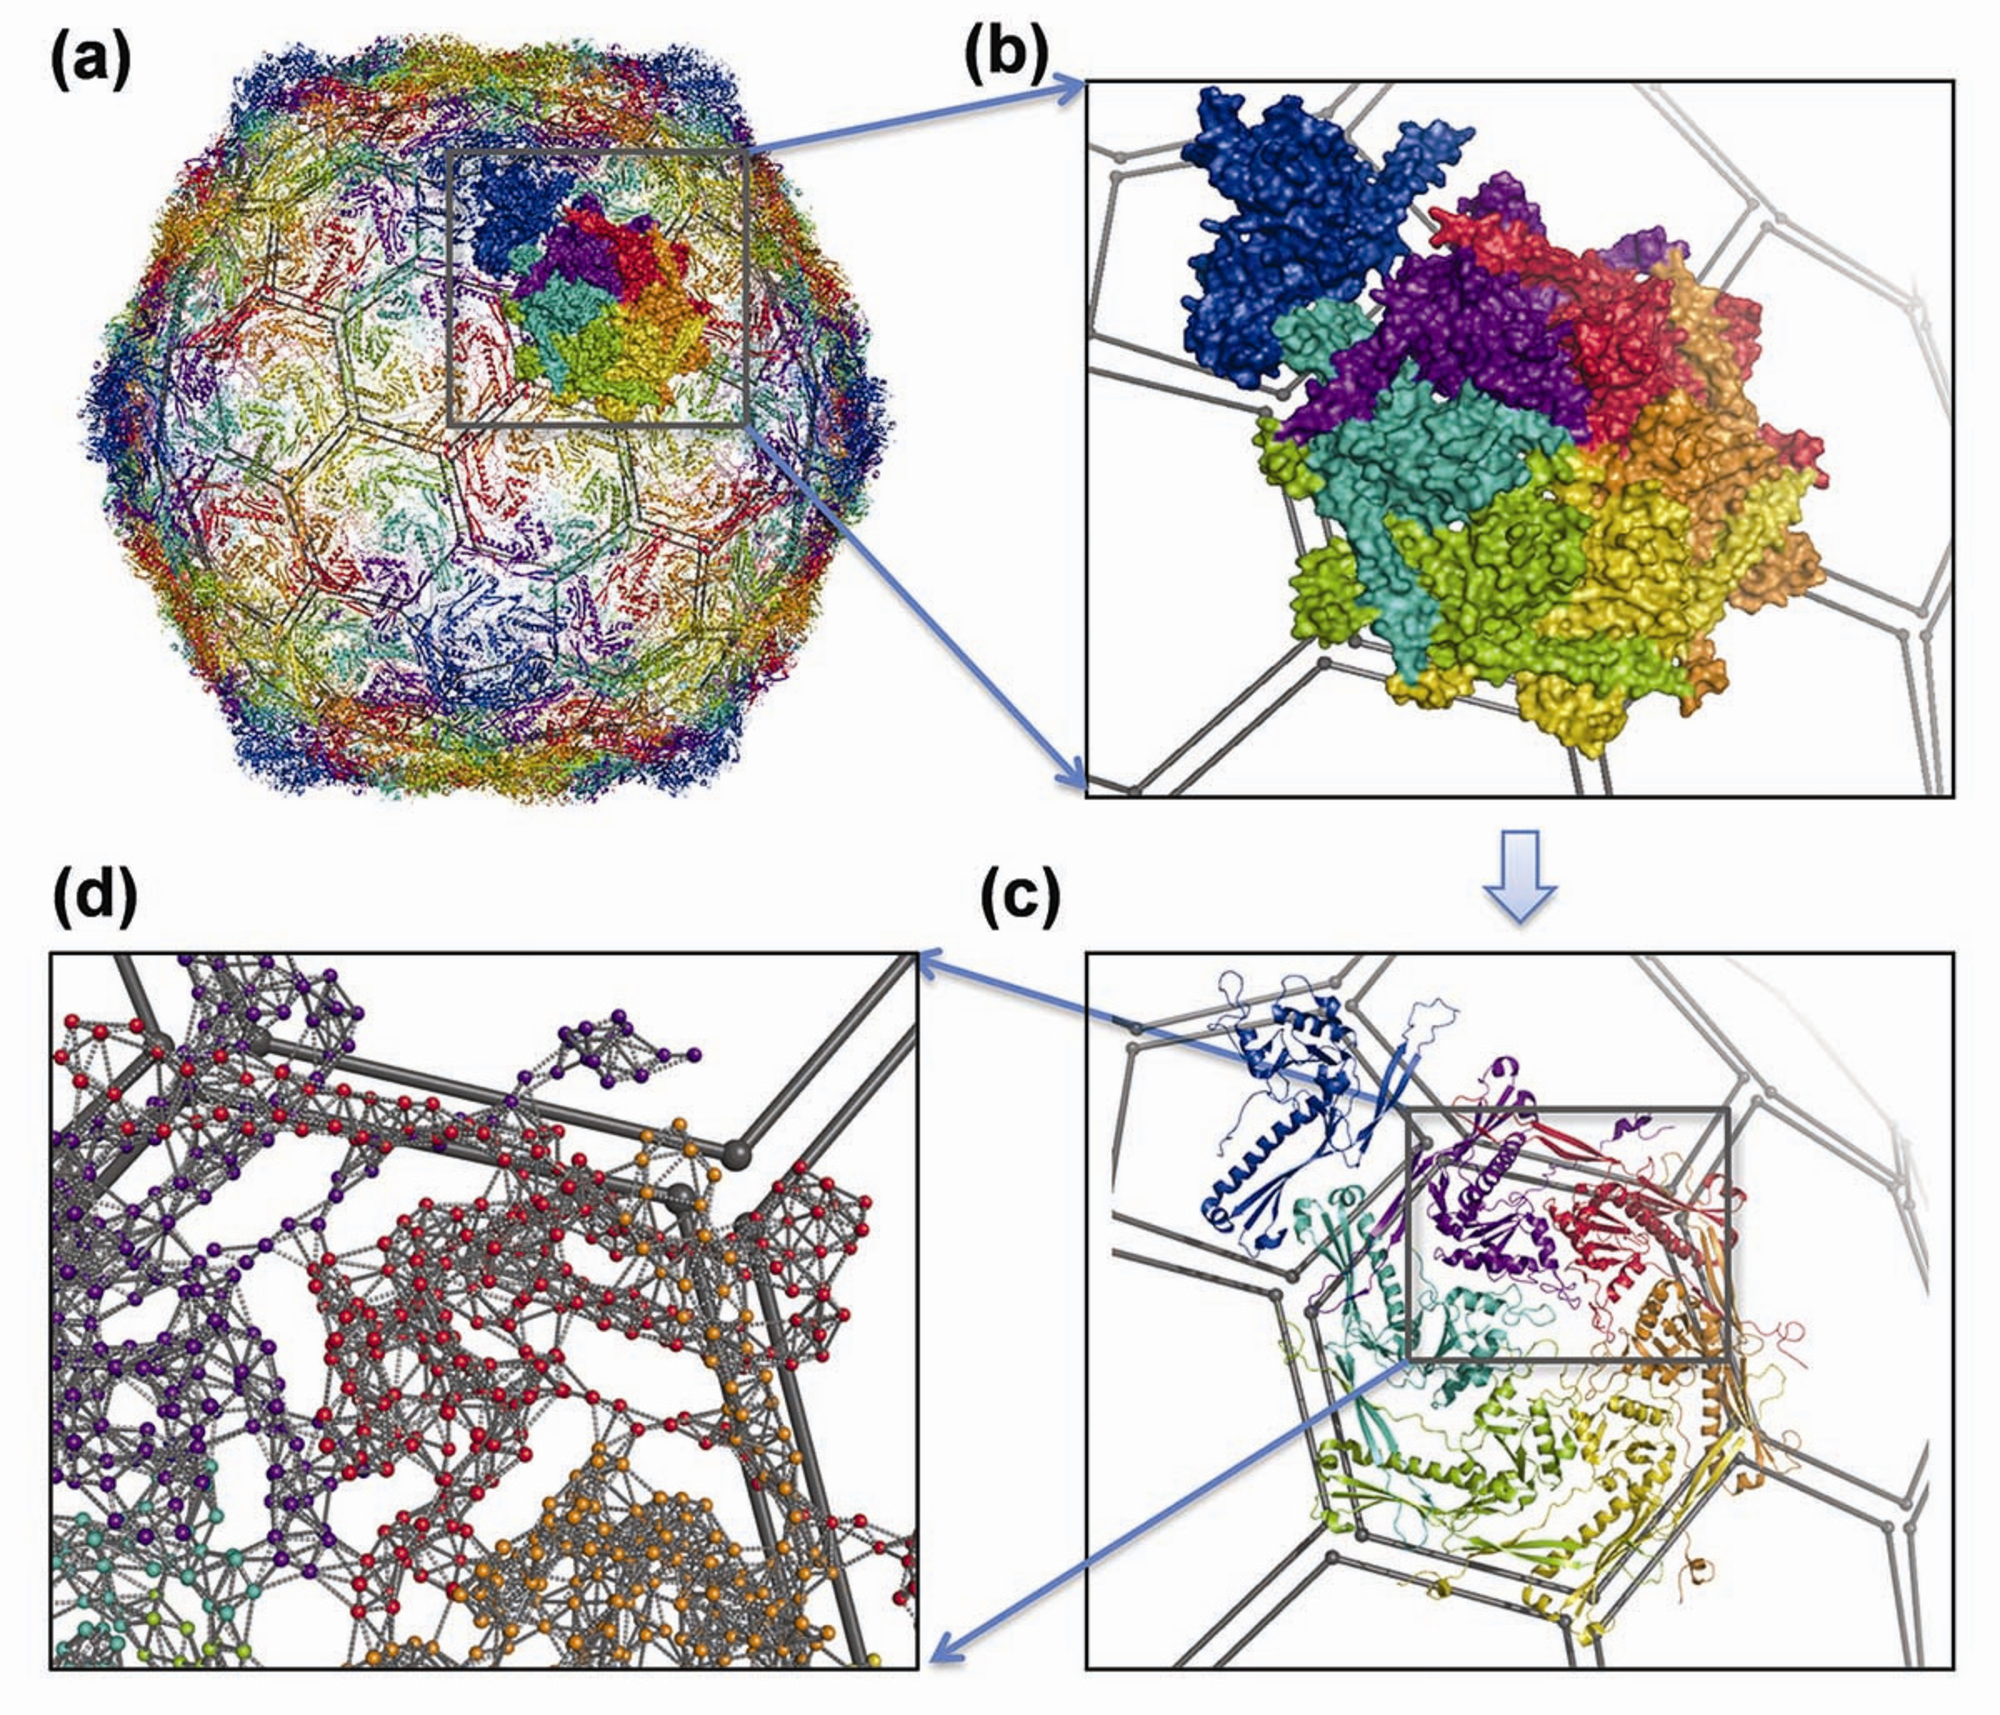
\includegraphics[scale=0.3]{Kap2/dibujo.pdf}%
\caption{ (a) Vista exterior de un c\'{a}pside v\'{i}rico HK97 coloreado por cada cadena, todas las prote\'{i}nas son id\'{e}nticas. (b) Vista del arreglo prote\'{i}nico en una cara del c\'{a}pside. (c) Vista de la estructura secundaria de las prote\'{i}nas (d) Esquema de cada prote\'{i}na mostrando cada uno de sus \'{a}tomos, las aristas de cada cara son carbonos $\alpha$ unidos por lados (ligaduras el\'{a}sticas). Tomado de \cite{Lezon2009ElasticViruses}.} \label{fig:pan}
\end{figure}
\subsubsection{Descripci\'{o}n Mec\'{a}nica del Modelo}

Consid\'{e}rese una biomol\'{e}cula con $N$ part\'{i}culas constituyentes, el tipo de constituyente depende del modelo apropiado para la biomol\'{e}cula, por ejemplo en las prote\'{i}nas como la BPTI, ver \cite{Gur2013GlobalPredictions.}, los constituyentes son los carbonos $\alpha$ de los amino\'{a}cidos.\\

La energ\'{i}a potencial $V$ que representa las interacciones entre los constituyentes de la biomol\'{e}cula, se puede expresar alrededor de las posiciones de equilibrio $\mathbf{q_0}=\mathbf{0}$ tal como describe la teor\'{i}a de peque\~{n}as oscilaciones, ver \cite{Goldstein2001ClassicalMechanics}:
\begin{equation}
V(q)=V(\mathbf{0})+\sum_{i=1}^n\frac{\partial V}{\partial q_i}q_i+\sum_{ij}^{n}\frac{\partial^2 V }{\partial q_i\partial q_j}q_i q_j+...
\end{equation}\label{eq:1}
Donde $q_i$ son los desplazamientos con respecto a las posiciones de equilibrio, $n$ es el n\'{u}mero de posibles desplazamientos en la biomol\'{e}cula. $V(\mathbf{0})$ es el potencial en equilibrio que por conveniencia puede ser calibrado a cero: $V(\mathbf{0})=0$. \\


El sistema se encuentra alrededor del equilibrio cuando las fuerzas generalizadas se anulan, esto es:
\begin{equation}
\frac{\partial V}{\partial q_i}=0
\end{equation}\label{eq:2}
En este tipo de casos como la energ\'{i}a se minimiza, se dice que hay un equilibrio estable. Para entender esto, sup\'{o}gase que la energ\'{i}a total, que en este caso es $E=T+V$ corresponde al punto de equilibrio donde los nodos no se mueven, es decir, $E=V_{min}$ (l\'{i}nea punteada de la figura \ref{fig:pot}). Ahora suponga que hay una incremento de la energ\'{i}a total en una cantidad $\Delta E$, este incremento generar\'{a} un aumento en la energ\'{i}a potencial, l\'{i}nea continua.  Si el sistema se desv\'{i}a de la posici\'{o}n de equilibrio, por conservaci\'{o}n de la energ\'{i}a y como $E=T+V$, la energ\'{i}a cin\'{e}tica disminuye. En un equilibrio inestable la energ\'{i}a cin\'{e}tica aumenta, alejando al sistema del equilibrio. \cite{Goldstein2001ClassicalMechanics} \\


\begin{figure}
\centering%
% GNUPLOT: LaTeX picture
\setlength{\unitlength}{0.240900pt}
\ifx\plotpoint\undefined\newsavebox{\plotpoint}\fi
\begin{picture}(1500,900)(0,0)
\sbox{\plotpoint}{\rule[-0.200pt]{0.400pt}{0.400pt}}%
\put(171.0,174.0){\rule[-0.200pt]{4.818pt}{0.400pt}}
\put(151,174){\makebox(0,0)[r]{$-0.4$}}
\put(1419.0,174.0){\rule[-0.200pt]{4.818pt}{0.400pt}}
\put(171.0,259.0){\rule[-0.200pt]{4.818pt}{0.400pt}}
\put(151,259){\makebox(0,0)[r]{$-0.2$}}
\put(1419.0,259.0){\rule[-0.200pt]{4.818pt}{0.400pt}}
\put(171.0,345.0){\rule[-0.200pt]{4.818pt}{0.400pt}}
\put(151,345){\makebox(0,0)[r]{$0$}}
\put(1419.0,345.0){\rule[-0.200pt]{4.818pt}{0.400pt}}
\put(171.0,431.0){\rule[-0.200pt]{4.818pt}{0.400pt}}
\put(151,431){\makebox(0,0)[r]{$0.2$}}
\put(1419.0,431.0){\rule[-0.200pt]{4.818pt}{0.400pt}}
\put(171.0,516.0){\rule[-0.200pt]{4.818pt}{0.400pt}}
\put(151,516){\makebox(0,0)[r]{$0.4$}}
\put(1419.0,516.0){\rule[-0.200pt]{4.818pt}{0.400pt}}
\put(171.0,602.0){\rule[-0.200pt]{4.818pt}{0.400pt}}
\put(151,602){\makebox(0,0)[r]{$0.6$}}
\put(1419.0,602.0){\rule[-0.200pt]{4.818pt}{0.400pt}}
\put(171.0,688.0){\rule[-0.200pt]{4.818pt}{0.400pt}}
\put(151,688){\makebox(0,0)[r]{$0.8$}}
\put(1419.0,688.0){\rule[-0.200pt]{4.818pt}{0.400pt}}
\put(171.0,773.0){\rule[-0.200pt]{4.818pt}{0.400pt}}
\put(151,773){\makebox(0,0)[r]{$1$}}
\put(1419.0,773.0){\rule[-0.200pt]{4.818pt}{0.400pt}}
\put(171.0,859.0){\rule[-0.200pt]{4.818pt}{0.400pt}}
\put(151,859){\makebox(0,0)[r]{$1.2$}}
\put(1419.0,859.0){\rule[-0.200pt]{4.818pt}{0.400pt}}
\put(171.0,131.0){\rule[-0.200pt]{0.400pt}{4.818pt}}
\put(171,90){\makebox(0,0){$0$}}
\put(171.0,839.0){\rule[-0.200pt]{0.400pt}{4.818pt}}
\put(488.0,131.0){\rule[-0.200pt]{0.400pt}{4.818pt}}
\put(488,90){\makebox(0,0){$0.5$}}
\put(488.0,839.0){\rule[-0.200pt]{0.400pt}{4.818pt}}
\put(805.0,131.0){\rule[-0.200pt]{0.400pt}{4.818pt}}
\put(805,90){\makebox(0,0){$1$}}
\put(805.0,839.0){\rule[-0.200pt]{0.400pt}{4.818pt}}
\put(1122.0,131.0){\rule[-0.200pt]{0.400pt}{4.818pt}}
\put(1122,90){\makebox(0,0){$1.5$}}
\put(1122.0,839.0){\rule[-0.200pt]{0.400pt}{4.818pt}}
\put(1439.0,131.0){\rule[-0.200pt]{0.400pt}{4.818pt}}
\put(1439,90){\makebox(0,0){$2$}}
\put(1439.0,839.0){\rule[-0.200pt]{0.400pt}{4.818pt}}
\put(171.0,131.0){\rule[-0.200pt]{0.400pt}{175.375pt}}
\put(171.0,131.0){\rule[-0.200pt]{305.461pt}{0.400pt}}
\put(1439.0,131.0){\rule[-0.200pt]{0.400pt}{175.375pt}}
\put(171.0,859.0){\rule[-0.200pt]{305.461pt}{0.400pt}}
\put(30,495){\makebox(0,0){$V(q)$}}
\put(805,29){\makebox(0,0){$q$}}
\put(171,773){\usebox{\plotpoint}}
\multiput(171.58,770.41)(0.493,-0.655){23}{\rule{0.119pt}{0.623pt}}
\multiput(170.17,771.71)(13.000,-15.707){2}{\rule{0.400pt}{0.312pt}}
\multiput(184.58,753.41)(0.493,-0.655){23}{\rule{0.119pt}{0.623pt}}
\multiput(183.17,754.71)(13.000,-15.707){2}{\rule{0.400pt}{0.312pt}}
\multiput(197.58,736.37)(0.492,-0.669){21}{\rule{0.119pt}{0.633pt}}
\multiput(196.17,737.69)(12.000,-14.685){2}{\rule{0.400pt}{0.317pt}}
\multiput(209.58,720.54)(0.493,-0.616){23}{\rule{0.119pt}{0.592pt}}
\multiput(208.17,721.77)(13.000,-14.771){2}{\rule{0.400pt}{0.296pt}}
\multiput(222.58,704.54)(0.493,-0.616){23}{\rule{0.119pt}{0.592pt}}
\multiput(221.17,705.77)(13.000,-14.771){2}{\rule{0.400pt}{0.296pt}}
\multiput(235.58,688.67)(0.493,-0.576){23}{\rule{0.119pt}{0.562pt}}
\multiput(234.17,689.83)(13.000,-13.834){2}{\rule{0.400pt}{0.281pt}}
\multiput(248.58,673.67)(0.493,-0.576){23}{\rule{0.119pt}{0.562pt}}
\multiput(247.17,674.83)(13.000,-13.834){2}{\rule{0.400pt}{0.281pt}}
\multiput(261.58,658.51)(0.492,-0.625){21}{\rule{0.119pt}{0.600pt}}
\multiput(260.17,659.75)(12.000,-13.755){2}{\rule{0.400pt}{0.300pt}}
\multiput(273.58,643.80)(0.493,-0.536){23}{\rule{0.119pt}{0.531pt}}
\multiput(272.17,644.90)(13.000,-12.898){2}{\rule{0.400pt}{0.265pt}}
\multiput(286.58,629.80)(0.493,-0.536){23}{\rule{0.119pt}{0.531pt}}
\multiput(285.17,630.90)(13.000,-12.898){2}{\rule{0.400pt}{0.265pt}}
\multiput(299.58,615.80)(0.493,-0.536){23}{\rule{0.119pt}{0.531pt}}
\multiput(298.17,616.90)(13.000,-12.898){2}{\rule{0.400pt}{0.265pt}}
\multiput(312.00,602.92)(0.497,-0.493){23}{\rule{0.500pt}{0.119pt}}
\multiput(312.00,603.17)(11.962,-13.000){2}{\rule{0.250pt}{0.400pt}}
\multiput(325.00,589.92)(0.497,-0.493){23}{\rule{0.500pt}{0.119pt}}
\multiput(325.00,590.17)(11.962,-13.000){2}{\rule{0.250pt}{0.400pt}}
\multiput(338.58,575.79)(0.492,-0.539){21}{\rule{0.119pt}{0.533pt}}
\multiput(337.17,576.89)(12.000,-11.893){2}{\rule{0.400pt}{0.267pt}}
\multiput(350.00,563.92)(0.539,-0.492){21}{\rule{0.533pt}{0.119pt}}
\multiput(350.00,564.17)(11.893,-12.000){2}{\rule{0.267pt}{0.400pt}}
\multiput(363.00,551.92)(0.539,-0.492){21}{\rule{0.533pt}{0.119pt}}
\multiput(363.00,552.17)(11.893,-12.000){2}{\rule{0.267pt}{0.400pt}}
\multiput(376.00,539.92)(0.590,-0.492){19}{\rule{0.573pt}{0.118pt}}
\multiput(376.00,540.17)(11.811,-11.000){2}{\rule{0.286pt}{0.400pt}}
\multiput(389.00,528.92)(0.590,-0.492){19}{\rule{0.573pt}{0.118pt}}
\multiput(389.00,529.17)(11.811,-11.000){2}{\rule{0.286pt}{0.400pt}}
\multiput(402.00,517.92)(0.543,-0.492){19}{\rule{0.536pt}{0.118pt}}
\multiput(402.00,518.17)(10.887,-11.000){2}{\rule{0.268pt}{0.400pt}}
\multiput(414.00,506.92)(0.590,-0.492){19}{\rule{0.573pt}{0.118pt}}
\multiput(414.00,507.17)(11.811,-11.000){2}{\rule{0.286pt}{0.400pt}}
\multiput(427.00,495.92)(0.652,-0.491){17}{\rule{0.620pt}{0.118pt}}
\multiput(427.00,496.17)(11.713,-10.000){2}{\rule{0.310pt}{0.400pt}}
\multiput(440.00,485.92)(0.652,-0.491){17}{\rule{0.620pt}{0.118pt}}
\multiput(440.00,486.17)(11.713,-10.000){2}{\rule{0.310pt}{0.400pt}}
\multiput(453.00,475.93)(0.728,-0.489){15}{\rule{0.678pt}{0.118pt}}
\multiput(453.00,476.17)(11.593,-9.000){2}{\rule{0.339pt}{0.400pt}}
\multiput(466.00,466.93)(0.669,-0.489){15}{\rule{0.633pt}{0.118pt}}
\multiput(466.00,467.17)(10.685,-9.000){2}{\rule{0.317pt}{0.400pt}}
\multiput(478.00,457.93)(0.728,-0.489){15}{\rule{0.678pt}{0.118pt}}
\multiput(478.00,458.17)(11.593,-9.000){2}{\rule{0.339pt}{0.400pt}}
\multiput(491.00,448.93)(0.824,-0.488){13}{\rule{0.750pt}{0.117pt}}
\multiput(491.00,449.17)(11.443,-8.000){2}{\rule{0.375pt}{0.400pt}}
\multiput(504.00,440.93)(0.824,-0.488){13}{\rule{0.750pt}{0.117pt}}
\multiput(504.00,441.17)(11.443,-8.000){2}{\rule{0.375pt}{0.400pt}}
\multiput(517.00,432.93)(0.824,-0.488){13}{\rule{0.750pt}{0.117pt}}
\multiput(517.00,433.17)(11.443,-8.000){2}{\rule{0.375pt}{0.400pt}}
\multiput(530.00,424.93)(0.874,-0.485){11}{\rule{0.786pt}{0.117pt}}
\multiput(530.00,425.17)(10.369,-7.000){2}{\rule{0.393pt}{0.400pt}}
\multiput(542.00,417.93)(0.950,-0.485){11}{\rule{0.843pt}{0.117pt}}
\multiput(542.00,418.17)(11.251,-7.000){2}{\rule{0.421pt}{0.400pt}}
\multiput(555.00,410.93)(0.950,-0.485){11}{\rule{0.843pt}{0.117pt}}
\multiput(555.00,411.17)(11.251,-7.000){2}{\rule{0.421pt}{0.400pt}}
\multiput(568.00,403.93)(1.123,-0.482){9}{\rule{0.967pt}{0.116pt}}
\multiput(568.00,404.17)(10.994,-6.000){2}{\rule{0.483pt}{0.400pt}}
\multiput(581.00,397.93)(1.123,-0.482){9}{\rule{0.967pt}{0.116pt}}
\multiput(581.00,398.17)(10.994,-6.000){2}{\rule{0.483pt}{0.400pt}}
\multiput(594.00,391.93)(1.033,-0.482){9}{\rule{0.900pt}{0.116pt}}
\multiput(594.00,392.17)(10.132,-6.000){2}{\rule{0.450pt}{0.400pt}}
\multiput(606.00,385.93)(1.378,-0.477){7}{\rule{1.140pt}{0.115pt}}
\multiput(606.00,386.17)(10.634,-5.000){2}{\rule{0.570pt}{0.400pt}}
\multiput(619.00,380.93)(1.378,-0.477){7}{\rule{1.140pt}{0.115pt}}
\multiput(619.00,381.17)(10.634,-5.000){2}{\rule{0.570pt}{0.400pt}}
\multiput(632.00,375.93)(1.378,-0.477){7}{\rule{1.140pt}{0.115pt}}
\multiput(632.00,376.17)(10.634,-5.000){2}{\rule{0.570pt}{0.400pt}}
\multiput(645.00,370.94)(1.797,-0.468){5}{\rule{1.400pt}{0.113pt}}
\multiput(645.00,371.17)(10.094,-4.000){2}{\rule{0.700pt}{0.400pt}}
\multiput(658.00,366.94)(1.797,-0.468){5}{\rule{1.400pt}{0.113pt}}
\multiput(658.00,367.17)(10.094,-4.000){2}{\rule{0.700pt}{0.400pt}}
\multiput(671.00,362.95)(2.472,-0.447){3}{\rule{1.700pt}{0.108pt}}
\multiput(671.00,363.17)(8.472,-3.000){2}{\rule{0.850pt}{0.400pt}}
\multiput(683.00,359.95)(2.695,-0.447){3}{\rule{1.833pt}{0.108pt}}
\multiput(683.00,360.17)(9.195,-3.000){2}{\rule{0.917pt}{0.400pt}}
\multiput(696.00,356.95)(2.695,-0.447){3}{\rule{1.833pt}{0.108pt}}
\multiput(696.00,357.17)(9.195,-3.000){2}{\rule{0.917pt}{0.400pt}}
\put(709,353.17){\rule{2.700pt}{0.400pt}}
\multiput(709.00,354.17)(7.396,-2.000){2}{\rule{1.350pt}{0.400pt}}
\multiput(722.00,351.95)(2.695,-0.447){3}{\rule{1.833pt}{0.108pt}}
\multiput(722.00,352.17)(9.195,-3.000){2}{\rule{0.917pt}{0.400pt}}
\put(735,348.67){\rule{2.891pt}{0.400pt}}
\multiput(735.00,349.17)(6.000,-1.000){2}{\rule{1.445pt}{0.400pt}}
\put(747,347.17){\rule{2.700pt}{0.400pt}}
\multiput(747.00,348.17)(7.396,-2.000){2}{\rule{1.350pt}{0.400pt}}
\put(760,345.67){\rule{3.132pt}{0.400pt}}
\multiput(760.00,346.17)(6.500,-1.000){2}{\rule{1.566pt}{0.400pt}}
\put(786,344.67){\rule{3.132pt}{0.400pt}}
\multiput(786.00,345.17)(6.500,-1.000){2}{\rule{1.566pt}{0.400pt}}
\put(773.0,346.0){\rule[-0.200pt]{3.132pt}{0.400pt}}
\put(811,344.67){\rule{3.132pt}{0.400pt}}
\multiput(811.00,344.17)(6.500,1.000){2}{\rule{1.566pt}{0.400pt}}
\put(799.0,345.0){\rule[-0.200pt]{2.891pt}{0.400pt}}
\put(837,345.67){\rule{3.132pt}{0.400pt}}
\multiput(837.00,345.17)(6.500,1.000){2}{\rule{1.566pt}{0.400pt}}
\put(850,347.17){\rule{2.700pt}{0.400pt}}
\multiput(850.00,346.17)(7.396,2.000){2}{\rule{1.350pt}{0.400pt}}
\put(863,348.67){\rule{2.891pt}{0.400pt}}
\multiput(863.00,348.17)(6.000,1.000){2}{\rule{1.445pt}{0.400pt}}
\multiput(875.00,350.61)(2.695,0.447){3}{\rule{1.833pt}{0.108pt}}
\multiput(875.00,349.17)(9.195,3.000){2}{\rule{0.917pt}{0.400pt}}
\put(888,353.17){\rule{2.700pt}{0.400pt}}
\multiput(888.00,352.17)(7.396,2.000){2}{\rule{1.350pt}{0.400pt}}
\multiput(901.00,355.61)(2.695,0.447){3}{\rule{1.833pt}{0.108pt}}
\multiput(901.00,354.17)(9.195,3.000){2}{\rule{0.917pt}{0.400pt}}
\multiput(914.00,358.61)(2.695,0.447){3}{\rule{1.833pt}{0.108pt}}
\multiput(914.00,357.17)(9.195,3.000){2}{\rule{0.917pt}{0.400pt}}
\multiput(927.00,361.61)(2.472,0.447){3}{\rule{1.700pt}{0.108pt}}
\multiput(927.00,360.17)(8.472,3.000){2}{\rule{0.850pt}{0.400pt}}
\multiput(939.00,364.60)(1.797,0.468){5}{\rule{1.400pt}{0.113pt}}
\multiput(939.00,363.17)(10.094,4.000){2}{\rule{0.700pt}{0.400pt}}
\multiput(952.00,368.60)(1.797,0.468){5}{\rule{1.400pt}{0.113pt}}
\multiput(952.00,367.17)(10.094,4.000){2}{\rule{0.700pt}{0.400pt}}
\multiput(965.00,372.59)(1.378,0.477){7}{\rule{1.140pt}{0.115pt}}
\multiput(965.00,371.17)(10.634,5.000){2}{\rule{0.570pt}{0.400pt}}
\multiput(978.00,377.59)(1.378,0.477){7}{\rule{1.140pt}{0.115pt}}
\multiput(978.00,376.17)(10.634,5.000){2}{\rule{0.570pt}{0.400pt}}
\multiput(991.00,382.59)(1.378,0.477){7}{\rule{1.140pt}{0.115pt}}
\multiput(991.00,381.17)(10.634,5.000){2}{\rule{0.570pt}{0.400pt}}
\multiput(1004.00,387.59)(1.033,0.482){9}{\rule{0.900pt}{0.116pt}}
\multiput(1004.00,386.17)(10.132,6.000){2}{\rule{0.450pt}{0.400pt}}
\multiput(1016.00,393.59)(1.123,0.482){9}{\rule{0.967pt}{0.116pt}}
\multiput(1016.00,392.17)(10.994,6.000){2}{\rule{0.483pt}{0.400pt}}
\multiput(1029.00,399.59)(1.123,0.482){9}{\rule{0.967pt}{0.116pt}}
\multiput(1029.00,398.17)(10.994,6.000){2}{\rule{0.483pt}{0.400pt}}
\multiput(1042.00,405.59)(0.950,0.485){11}{\rule{0.843pt}{0.117pt}}
\multiput(1042.00,404.17)(11.251,7.000){2}{\rule{0.421pt}{0.400pt}}
\multiput(1055.00,412.59)(0.950,0.485){11}{\rule{0.843pt}{0.117pt}}
\multiput(1055.00,411.17)(11.251,7.000){2}{\rule{0.421pt}{0.400pt}}
\multiput(1068.00,419.59)(0.874,0.485){11}{\rule{0.786pt}{0.117pt}}
\multiput(1068.00,418.17)(10.369,7.000){2}{\rule{0.393pt}{0.400pt}}
\multiput(1080.00,426.59)(0.824,0.488){13}{\rule{0.750pt}{0.117pt}}
\multiput(1080.00,425.17)(11.443,8.000){2}{\rule{0.375pt}{0.400pt}}
\multiput(1093.00,434.59)(0.824,0.488){13}{\rule{0.750pt}{0.117pt}}
\multiput(1093.00,433.17)(11.443,8.000){2}{\rule{0.375pt}{0.400pt}}
\multiput(1106.00,442.59)(0.824,0.488){13}{\rule{0.750pt}{0.117pt}}
\multiput(1106.00,441.17)(11.443,8.000){2}{\rule{0.375pt}{0.400pt}}
\multiput(1119.00,450.59)(0.728,0.489){15}{\rule{0.678pt}{0.118pt}}
\multiput(1119.00,449.17)(11.593,9.000){2}{\rule{0.339pt}{0.400pt}}
\multiput(1132.00,459.59)(0.669,0.489){15}{\rule{0.633pt}{0.118pt}}
\multiput(1132.00,458.17)(10.685,9.000){2}{\rule{0.317pt}{0.400pt}}
\multiput(1144.00,468.59)(0.728,0.489){15}{\rule{0.678pt}{0.118pt}}
\multiput(1144.00,467.17)(11.593,9.000){2}{\rule{0.339pt}{0.400pt}}
\multiput(1157.00,477.58)(0.652,0.491){17}{\rule{0.620pt}{0.118pt}}
\multiput(1157.00,476.17)(11.713,10.000){2}{\rule{0.310pt}{0.400pt}}
\multiput(1170.00,487.58)(0.652,0.491){17}{\rule{0.620pt}{0.118pt}}
\multiput(1170.00,486.17)(11.713,10.000){2}{\rule{0.310pt}{0.400pt}}
\multiput(1183.00,497.58)(0.590,0.492){19}{\rule{0.573pt}{0.118pt}}
\multiput(1183.00,496.17)(11.811,11.000){2}{\rule{0.286pt}{0.400pt}}
\multiput(1196.00,508.58)(0.543,0.492){19}{\rule{0.536pt}{0.118pt}}
\multiput(1196.00,507.17)(10.887,11.000){2}{\rule{0.268pt}{0.400pt}}
\multiput(1208.00,519.58)(0.590,0.492){19}{\rule{0.573pt}{0.118pt}}
\multiput(1208.00,518.17)(11.811,11.000){2}{\rule{0.286pt}{0.400pt}}
\multiput(1221.00,530.58)(0.590,0.492){19}{\rule{0.573pt}{0.118pt}}
\multiput(1221.00,529.17)(11.811,11.000){2}{\rule{0.286pt}{0.400pt}}
\multiput(1234.00,541.58)(0.539,0.492){21}{\rule{0.533pt}{0.119pt}}
\multiput(1234.00,540.17)(11.893,12.000){2}{\rule{0.267pt}{0.400pt}}
\multiput(1247.00,553.58)(0.539,0.492){21}{\rule{0.533pt}{0.119pt}}
\multiput(1247.00,552.17)(11.893,12.000){2}{\rule{0.267pt}{0.400pt}}
\multiput(1260.58,565.00)(0.492,0.539){21}{\rule{0.119pt}{0.533pt}}
\multiput(1259.17,565.00)(12.000,11.893){2}{\rule{0.400pt}{0.267pt}}
\multiput(1272.00,578.58)(0.497,0.493){23}{\rule{0.500pt}{0.119pt}}
\multiput(1272.00,577.17)(11.962,13.000){2}{\rule{0.250pt}{0.400pt}}
\multiput(1285.00,591.58)(0.497,0.493){23}{\rule{0.500pt}{0.119pt}}
\multiput(1285.00,590.17)(11.962,13.000){2}{\rule{0.250pt}{0.400pt}}
\multiput(1298.58,604.00)(0.493,0.536){23}{\rule{0.119pt}{0.531pt}}
\multiput(1297.17,604.00)(13.000,12.898){2}{\rule{0.400pt}{0.265pt}}
\multiput(1311.58,618.00)(0.493,0.536){23}{\rule{0.119pt}{0.531pt}}
\multiput(1310.17,618.00)(13.000,12.898){2}{\rule{0.400pt}{0.265pt}}
\multiput(1324.58,632.00)(0.493,0.536){23}{\rule{0.119pt}{0.531pt}}
\multiput(1323.17,632.00)(13.000,12.898){2}{\rule{0.400pt}{0.265pt}}
\multiput(1337.58,646.00)(0.492,0.625){21}{\rule{0.119pt}{0.600pt}}
\multiput(1336.17,646.00)(12.000,13.755){2}{\rule{0.400pt}{0.300pt}}
\multiput(1349.58,661.00)(0.493,0.576){23}{\rule{0.119pt}{0.562pt}}
\multiput(1348.17,661.00)(13.000,13.834){2}{\rule{0.400pt}{0.281pt}}
\multiput(1362.58,676.00)(0.493,0.576){23}{\rule{0.119pt}{0.562pt}}
\multiput(1361.17,676.00)(13.000,13.834){2}{\rule{0.400pt}{0.281pt}}
\multiput(1375.58,691.00)(0.493,0.616){23}{\rule{0.119pt}{0.592pt}}
\multiput(1374.17,691.00)(13.000,14.771){2}{\rule{0.400pt}{0.296pt}}
\multiput(1388.58,707.00)(0.493,0.616){23}{\rule{0.119pt}{0.592pt}}
\multiput(1387.17,707.00)(13.000,14.771){2}{\rule{0.400pt}{0.296pt}}
\multiput(1401.58,723.00)(0.492,0.669){21}{\rule{0.119pt}{0.633pt}}
\multiput(1400.17,723.00)(12.000,14.685){2}{\rule{0.400pt}{0.317pt}}
\multiput(1413.58,739.00)(0.493,0.655){23}{\rule{0.119pt}{0.623pt}}
\multiput(1412.17,739.00)(13.000,15.707){2}{\rule{0.400pt}{0.312pt}}
\multiput(1426.58,756.00)(0.493,0.655){23}{\rule{0.119pt}{0.623pt}}
\multiput(1425.17,756.00)(13.000,15.707){2}{\rule{0.400pt}{0.312pt}}
\put(824.0,346.0){\rule[-0.200pt]{3.132pt}{0.400pt}}
\put(171,345){\usebox{\plotpoint}}
\put(171.00,345.00){\usebox{\plotpoint}}
\put(191.76,345.00){\usebox{\plotpoint}}
\put(212.51,345.00){\usebox{\plotpoint}}
\put(233.27,345.00){\usebox{\plotpoint}}
\put(254.02,345.00){\usebox{\plotpoint}}
\put(274.78,345.00){\usebox{\plotpoint}}
\put(295.53,345.00){\usebox{\plotpoint}}
\put(316.29,345.00){\usebox{\plotpoint}}
\put(337.04,345.00){\usebox{\plotpoint}}
\put(357.80,345.00){\usebox{\plotpoint}}
\put(378.56,345.00){\usebox{\plotpoint}}
\put(399.31,345.00){\usebox{\plotpoint}}
\put(420.07,345.00){\usebox{\plotpoint}}
\put(440.82,345.00){\usebox{\plotpoint}}
\put(461.58,345.00){\usebox{\plotpoint}}
\put(482.33,345.00){\usebox{\plotpoint}}
\put(503.09,345.00){\usebox{\plotpoint}}
\put(523.84,345.00){\usebox{\plotpoint}}
\put(544.60,345.00){\usebox{\plotpoint}}
\put(565.35,345.00){\usebox{\plotpoint}}
\put(586.11,345.00){\usebox{\plotpoint}}
\put(606.87,345.00){\usebox{\plotpoint}}
\put(627.62,345.00){\usebox{\plotpoint}}
\put(648.38,345.00){\usebox{\plotpoint}}
\put(669.13,345.00){\usebox{\plotpoint}}
\put(689.89,345.00){\usebox{\plotpoint}}
\put(710.64,345.00){\usebox{\plotpoint}}
\put(731.40,345.00){\usebox{\plotpoint}}
\put(752.15,345.00){\usebox{\plotpoint}}
\put(772.91,345.00){\usebox{\plotpoint}}
\put(793.66,345.00){\usebox{\plotpoint}}
\put(814.42,345.00){\usebox{\plotpoint}}
\put(835.18,345.00){\usebox{\plotpoint}}
\put(855.93,345.00){\usebox{\plotpoint}}
\put(876.69,345.00){\usebox{\plotpoint}}
\put(897.44,345.00){\usebox{\plotpoint}}
\put(918.20,345.00){\usebox{\plotpoint}}
\put(938.95,345.00){\usebox{\plotpoint}}
\put(959.71,345.00){\usebox{\plotpoint}}
\put(980.46,345.00){\usebox{\plotpoint}}
\put(1001.22,345.00){\usebox{\plotpoint}}
\put(1021.98,345.00){\usebox{\plotpoint}}
\put(1042.73,345.00){\usebox{\plotpoint}}
\put(1063.49,345.00){\usebox{\plotpoint}}
\put(1084.24,345.00){\usebox{\plotpoint}}
\put(1105.00,345.00){\usebox{\plotpoint}}
\put(1125.75,345.00){\usebox{\plotpoint}}
\put(1146.51,345.00){\usebox{\plotpoint}}
\put(1167.26,345.00){\usebox{\plotpoint}}
\put(1188.02,345.00){\usebox{\plotpoint}}
\put(1208.77,345.00){\usebox{\plotpoint}}
\put(1229.53,345.00){\usebox{\plotpoint}}
\put(1250.29,345.00){\usebox{\plotpoint}}
\put(1271.04,345.00){\usebox{\plotpoint}}
\put(1291.80,345.00){\usebox{\plotpoint}}
\put(1312.55,345.00){\usebox{\plotpoint}}
\put(1333.31,345.00){\usebox{\plotpoint}}
\put(1354.06,345.00){\usebox{\plotpoint}}
\put(1374.82,345.00){\usebox{\plotpoint}}
\put(1395.57,345.00){\usebox{\plotpoint}}
\put(1416.33,345.00){\usebox{\plotpoint}}
\put(1437.09,345.00){\usebox{\plotpoint}}
\put(1439,345){\usebox{\plotpoint}}
\sbox{\plotpoint}{\rule[-0.400pt]{0.800pt}{0.800pt}}%
\put(171,474){\usebox{\plotpoint}}
\put(171.0,474.0){\rule[-0.400pt]{305.461pt}{0.800pt}}
\sbox{\plotpoint}{\rule[-0.200pt]{0.400pt}{0.400pt}}%
\put(171.0,131.0){\rule[-0.200pt]{0.400pt}{175.375pt}}
\put(171.0,131.0){\rule[-0.200pt]{305.461pt}{0.400pt}}
\put(1439.0,131.0){\rule[-0.200pt]{0.400pt}{175.375pt}}
\put(171.0,859.0){\rule[-0.200pt]{305.461pt}{0.400pt}}
\end{picture}
%
\put(-830,330){$E$}
\put(-950,480){$E+\Delta E$}
\put(-400,390){$T$}
\put(-405,345){\vector(0,1){130}}
\put(-280,410){$T$}
\put(-300,375){\vector(0,1){100}}
\caption{Potencial en funci\'{o}n de la posici\'{o}n y energ\'{i}a total $E$} \label{fig:pot}
\end{figure}

Considerando la condici\'{o}n de equilibrio \eqref{eq:2} y despreciando desplazamientos de orden superior se tiene que:
\begin{equation}
V(\mathbf{q})=\sum_{i,j=1}^{n}\frac{\partial^2 V }{\partial q_i\partial q_j}q_i q_j
\end{equation}\label{eq:3}

Donde se identifican las constantes el\'{a}sticas como:
\begin{equation}
U_{ij}=\frac{\partial^2 V }{\partial q_i\partial q_j}
\end{equation}\label{eq:4}

En t\'{e}rminos matriciales el potencial se puede escribir como:
\begin{equation}
V(\mathbf{q})=\mathbf{q}^t\mathbf{U}\mathbf{q}
\end{equation}\label{eq:5}
En la ecuaci\'{o}n \eqref{eq:5} $\mathbf{q}$ es el vector columna formado por los desplazamientos de las posiciones de equilibrio para cada constituyente, i. e., $\mathbf{q}^t=(q_1,q_2,...q_n)$. Por otro lado la matriz de constantes el\'{a}sticas $\mathbf{H}$, es una matriz sim\'{e}trica debido a que la fuerza generalizada se considera conservativa, lo cual permite intercambiar el orden de las derivadas parciales.\\

Para las peque\~{n}as oscilaciones, no existen ligaduras dependientes expl\'{i}citamente de el tiempo (holon\'{o}micas) luego, la eneg\'{i}a cin\'{e}tica de los constituyentes s\'{o}lo depender\'{a} de los cuadrados de las velocidades generalizadas:
\begin{equation}
T=\frac{1}{2}\mathbf{q}^t\mathbf{M}\mathbf{q}
\end{equation}\label{eq:6}
Donde $\mathbf{M}$ es la masa generalizada, la cual se expresa en t\'{e}rminos de los factores de escala entre sistemas coordenados:
\begin{equation}
M_{jk}=\sum_{i=1}^{N} m_{i}\frac{\partial \mathbf{r_{i}} }{\partial q_j}\cdot\frac{\partial \mathbf{r_{i}} }{\partial q_k}
\end{equation}\label{eq:7}
La forma en que se escribir\'{a}n los elementos de la masa del sistema depende de la transformaci\'{o}n aplicada. Por ejemplo, en una dimensi\'{o}n las componentes de $\mathbf{q}$ se definen como:
\begin{equation}
q_i=x_i-x_{i0}
\end{equation}\label{eq:8}
En \eqref{eq:8} $x_i$ es la posici\'{o}n variable de la part\'{i}cula $i$ con respecto a un sistema fijo y $x_{i0}$ su posici\'{o}n de equilibrio. Para este caso particular \eqref{eq:7} se convierte en:
\begin{eqnarray}
M_{jk}&=&\sum_{i=1}^{N} m_{i} \delta_{ij}\delta_{ik}\nonumber \\
M_{jk}&=&m_{j} \delta_{jk}
\end{eqnarray}\label{eq:9}
La equaci\'{o}n \eqref{eq:9} dice que la matriz $\mathbf{M}$ es una matriz diagonal cuyas componentes son las masas del sistema.\\
En tres dimensiones, como es nuestro caso real, la transformaci\'{o}n depender\'{a} del modelo escogido. Exceptuando el modelo de redes gaussianas (Gaussian Network Model que por sus siglas en ingl\'{e}s es GNM) la transformaci\'{o}n de coordenadas va de $\mathbf{r}_{i}$ posiciones con $i=1,2,...,N$ ($3N$ coordenadas) a $q_j$ coordenadas $j=1,2,..,3N$:
\begin{equation*}
\mathbf{r}_{i}\longrightarrow q_{j}
\end{equation*}
Con
\begin{equation*}
i=1,2,...,N\mbox{  }j=1,2,..,3N
\end{equation*}
Por cada componente en cartesianas:
\begin{eqnarray}
\begin{array}{cccccc}
q_1=x_1-x_{10}&q_4=x_2-x_{20}&\cdots &q_{3i-2}=x_i-x_{i0}&\cdots &q_{3N-2}=x_N-x_{N0} \\
q_2=y_1-y_{10}&q_5=y_2-y_{20}&\cdots &q_{3i-1}=y_i-y_{i0}&\cdots &q_{3N-1}=y_N-y_{N0}\\
q_3=z_1-z_{10}&q_6=z_2-z_{20}&\cdots &q_{3i}=z_i-z_{i0}&\cdots &q_{3N}=z_N-z_{N0}\\
\end{array}
\end{eqnarray}\label{eq:10}
Para esta transformaci\'{o}n, \eqref{eq:7} se convierte en:
\begin{eqnarray}
M_{jk}&=&\sum_{i=1}^{N} m_{i}\left( \delta_{i,3j-2}\delta_{jk}+\delta_{i,3j-1}\delta_{jk}+  \delta_{i,3j}\delta_{jk}\right)\nonumber \\
M_{jk}&=&m_{3j-2}\delta_{jk}+m_{3j-1}\delta_{jk}+m_{3j}\delta_{jk} \nonumber \\
M_{jk}&=&\left( m_{3j-2}+m_{3j-1}+m_{3j} \right) \delta_{jk}
\end{eqnarray}\label{eq:11}
En \eqref{eq:11} debe resaltarse que para $j=k=3N$, el elemento de matriz $M_{3N,3N}$ requiere las masas $m_{3(3N)-2}=m_{9N-2}$, $m_{3(3N)-1}=m_{9N-1}$ y $m_{3(3N)}=m_{9N}$, sin embargo ! no hay $9N$ masas!, el n\'{u}mero de masas es el mismo n\'{u}mero de nodos: $N$, entonces, para poder calcular la matriz $\mathbf{M}$ es necesario definir lo siguiente:
\begin{equation}
m_{N+1},m_{N+2},...,m_{3N}=0
\end{equation}\label{eq:12}
Como a partir de $N+1$ las masas son nulas, la matriz de masa (que es diagonal) tiene elementos nulos si  
\begin{eqnarray*}
3j-2=N+1\\
j=\frac{N+3}{3} \\
\end{eqnarray*}
Como no siempre $N$ es m\'{u}ltiplo de 3, se escoge el entero menor que este m\'{a}s cerca al valor:
\begin{equation}
j=\left \lfloor\frac{N+3}{3}\right \rfloor
\end{equation}\label{eq:13}
\paragraph{Ecuaci\'{o}n de Movimiento}
El sistema satisface la ecuaci\'{o}n de un oscilador arm\'{o}nico, lo cual se muestra para las peque\~{n}as oscilaciones en \cite[Chapter~6]{Goldstein2001ClassicalMechanics} o puede ser revisado en el anexo \ref{AnexoA}:
\begin{equation}
\mathbf{M}\ddot{\mathbf{q}}+\mathbf{U}\mathbf{q}=\mathbf{0}
\end{equation}\label{eq:14}
Para convertir la ecuaci\'{o}n a la forma est\'{a}ndar se usan las coordenadas de masa ponderada (en ingl\'{e}s mass-weighted coordinates) las cuales cambian la escala en la que se mide la posici\'{o}n:
\begin{eqnarray}
\mathbf{q'}&=&\mathbf{M}^{1/2}\mathbf{q}\\
\mathbf{K}&=&\mathbf{M}^{-1/2}\mathbf{U}\mathbf{M}^{-1/2}
\end{eqnarray}\label{eq:15}
Reemplazando dichas transformaciones en la ecuaci\'{o}n de movimiento se obtiene:
\begin{equation}
\ddot{\mathbf{q'}}+\mathbf{K}\mathbf{q'}=\mathbf{0}
\end{equation}\label{eq:16}
El efecto que tienen las coordenadas de masa ponderada sobre la energias cin\'{e}tica  es el de desaparecer la dependencia con la matriz de masas del sistema, que como se vi\'{o} puede resultar en una expresi\'{o}n tediosa. Las energias cin\'{e}tica y potencial en las nuevas coordenadas son:
\begin{eqnarray}
T&=&\frac{1}{2}\mathbf{q}^t\mathbf{M}\mathbf{q} \nonumber \\
T&=&\frac{1}{2}\mathbf{\dot{r}}^t\mathbf{M^{-1/2}}^t\mathbf{M}\mathbf{M^{1/2}}\mathbf{\dot{r}}\nonumber \\
T&=&\frac{1}{2}\mathbf{\dot{r}}^t \mathbf{\dot{r}}
\end{eqnarray}\label{eq:19}
\begin{eqnarray}
V(\mathbf{q})&=&\mathbf{q}^t\mathbf{U}\mathbf{q} \nonumber \\
V(\mathbf{q})&=&\mathbf{r}^t\mathbf{M^{-1/2}}^t\mathbf{U}\mathbf{M^{1/2}}\mathbf{r} \nonumber \\
V(\mathbf{q})&=&\mathbf{r}^t\mathbf{K}\mathbf{r}
\end{eqnarray}\label{eq:20}
Una soluci\'{o}n (de prueba) a la ecuaci\'{o}n de movimiento es la oscilatoria, en la cual los constituyentes de la biomol\'{e}cula tienen la misma frecuencia $\omega$:
\begin{equation}
\mathbf{q'}=\mathbf{a}e^{i\omega t}
\end{equation}\label{eq:17}
El vector $\mathbf{a}$ es denominado vector de amplitudes debido a que cada una de sus componentes corresponde a las amplitudes de cada mon\'{o}mero. Sus valores son fijos en el tiempo.\\

Al reemplazar la soluci\'{o}n de prueba en la ecuaci\'{o}n \eqref{eq:16} se convierte en un problema de autovalores y autovectores:
\begin{eqnarray}
\ddot{\mathbf{q'}}&=&-\mathbf{K}\mathbf{q'} \nonumber \\
\omega^2\mathbf{a}&=&\mathbf{K}\mathbf{a} \nonumber \\
\lambda_{k}\mathbf{a_{k}}&=&\mathbf{K}\mathbf{a_{k}}
\end{eqnarray}\label{eq:18}
En \eqref{eq:18} se ha definido $\lambda=\omega^2$ y posteriormente se ha agregado el sub\'{i}ndice $k$ para distinguir cada uno de los autovalores y autovectores que se encuentren en el problema \eqref{eq:18}.\\
Cuando cada uno de los mon\'{o}meros tiene la misma frecuencia, a cada frecuencia le corresponde un vector de amplitudes $\mathbf{a}$, cada uno de estos posibles vectores se les conoce como un \textit{modo normal de oscilaci\'{o}n}.
\subsubsection{Ensamble Estad\'{i}stico}
Cuando el sistema (biomol\'{e}cula) se encuentre a temperaturas fisiol\'{o}gicas, el sistema  s\'{o}lo intercambiar\'{a} calor con los alrededores (ba\~{n}o t\'{e}rmico). Sin embargo, se ha demostrado  que a esta temperatura, la aproximaci\'{o}n arm\'{o}nica falla, presentando m\'{u}ltiples m\'{i}nimos y no uno solo. Como \'{u}nicamente hay intercambio de energ\'{i}a y se trabaja a temperatura fisiol\'{o}gica, la estad\'{i}stica apropidada es la del ensamble can\'{o}nico . En el ensamble  can\'{o}nico se sigue la distribuci\'{o} de probabilidad de Boltzmann:
\begin{equation}
p=\frac{\exp(-E_s/k_BT)}{Z}
\end{equation}\label{eq:21}
Donde $E_s$ es la energ\'{i}a del sistema y $Z$ la funci\'{o}n de partici\'{o}n. La funci\'{o}n de partici\'{o}n es el factor de normalizaci\'{o}n de la densidad de probabilidad y cuenta todos los posibles microestados a temperatura constante:
\begin{equation}
Z=\int \mathrm{d}^n p\mathrm{d}^n q \exp \left [-H(\mathbf{p},\mathbf{q})/k_BT \right]
\end{equation}\label{eq:22}
Ha de notarse que la funci\'{o}n de partici\'{o}n en \eqref{eq:22} desacopla los momentos y las posiciones, ya que el hamiltoniano est\'{a} dado por la f\'{o}rmula $H=T+V$,  
\subsubsection{Modelo de Redes Gaussianas (GNM)}
\subsubsection{Modelos de Redes Anisotr\'{o}picas (ANM)}
\subsection{An\'{a}lisis de Modos Normales Est\'{a}ndar (NMA)}
Describe un sistema oscilatorio en el que todos los constituyentes del sistema oscilan sinusoidalmente y con la misma frecuencia.
\subsection{An\'{a}lisis por Componentes Principales (PCA)}
\section{Movimientos Locales}
Hace referencia a las simulaciones en las que se incluyen todos los \'{a}tomos junto con las interacciones presentes, es decir, en las que se analizan los \textit{cambios locales}. Estas se pueden simular a un orden de magnitud de los nanosegundos en una m\'{a}quina usual, al respecto ver \cite{Gur2013GlobalPredictions.}.

Como caso particular se pueden tomar los potenciales usados en \cite{Amber2016AmberManual}, que siguen el modelo de Amber. El modelo de Amber tiene en cuenta las contribuciones debidas a:
 \begin{itemize}
\item Interacciones intermoleculares: Son las producidas por los enlaces covalentes entre grupos de \'{a}tomos, las de valencia y las torsiones.
\item Interacciones entre pares: Lennard Jones, electrost\'{a}tico.
\end{itemize}

\subsubsection{An\'{a}lisis por Componentes Principales}

\begin{itemize}
\item 
\end{itemize}
